\documentclass[french]{article}
\usepackage{babel}
\usepackage{fullpage}
\usepackage[utf8]{inputenc}
\usepackage[T1]{fontenc}
\usepackage{graphicx}
\usepackage{hyperref}
\usepackage{listings}


%
\def\frenchcontentsname{Sommaire}
%
\begin{document}

\begin{titlepage}
 \begin{sffamily}
  \begin{center}
            
\includegraphics[scale=0.04]{image/ubx-logo.png}
            \\[2cm]
        
    
    {\huge \bfseries Mémoire du Projet de programmation -\\ Corewar\\[0.5cm] }

    \rule{\linewidth}{.5pt}
    \\[2cm]

    \begin{minipage}{0.4\textwidth}
      \begin{flushleft} \large
        \author{}Étudiants : \item  Frédéric CHIPOT  \item Florian DAYRE \item Louis DUPLANTIER\\ \item  Alex FOURNIER\\ \item Gael HALNAUT
            
      \end{flushleft}
    \end{minipage}
    \begin{minipage}{0.4\textwidth}
      \begin{flushright} \large
        \emph{}\\  \textsc{}
      \end{flushright}
    \end{minipage}

    \vfill

    {\large }

  \end{center}
  \end{sffamily}
  
\end{titlepage}

\tableofcontents{}
\newpage

\section{Le contexte}
    \subsection{Introduction à Corewar}
        \paragraph{}Corewar est un jeu de contrôle d'espace mémoire, développé en 1984 par D. G. Jones et A. Dewdney. L’idée de Corewar provient des premiers vers informatiques créés au début des années 1970 par B. Thomas et R. Tomlinson. Le jeu se déroule dans une machine virtuelle, appelée MARS (Memory Array Redcode Simulator), dans laquelle s'affrontent des programmes, appelés guerriers. Le but du jeu est d’être le dernier programme en cours d’exécution.\\
    	Le combat se déroule de la manière suivante : un espace de départ est attribué à chaque programme, puis MARS va exécuter les instructions de chaque guerrier à tour de rôle. Lorsqu’un programme exécute une instruction particulière (DAT), cela tue le processus l’exécutant. Lorsqu’il n’a plus de processus, le programme meurt. Le combat prend fin lorsqu'il ne reste plus qu'un seul guerrier en vie, ou lorsque la totalité des tours a été joué. \\
    	Les guerriers se composent  d'une suite d’instructions (tâches, décrites ci-dessous) stockées dans la mémoire commune. Ils sont écrits en Redcode, un langage de programmation propre à Corewar ressemblant à un langage assembleur. Le terrain d’affrontements des programmes est un espace mémoire cyclique de taille "coresize", variable selon le mode de jeu, sans adressage absolu. Cet espace mémoire se compose au préalable d’instructions DAT. \\
        
        Un guerrier se décompose en une succession de lignes de code, chaque ligne comportant les éléments suivants : 
        \begin{itemize}
            \item Une instruction : 
                \begin{figure}[!h]
                    \centering 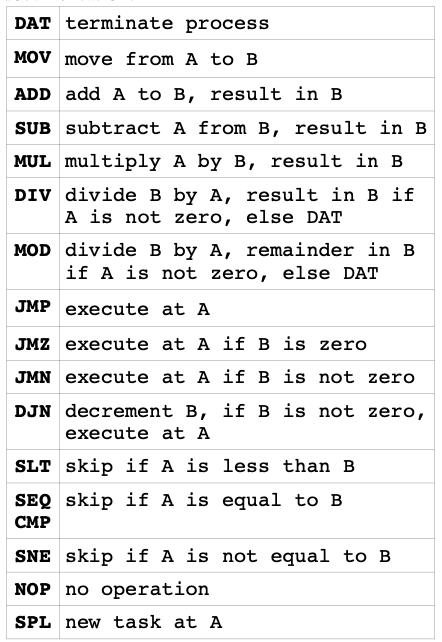
\includegraphics[scale=0.4]{image/instruction.png}
                    \caption{Liste des différentes instructions}
                \end{figure}
            \newpage
            \item Un modifieur pour l'instruction :
                \begin{figure}[!h]
                    \centering 
                    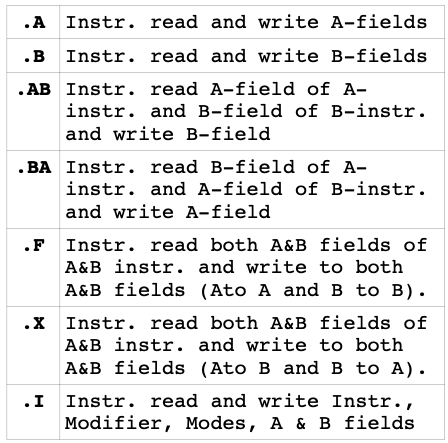
\includegraphics[scale=0.4]{image/modifieur.png}
                    \caption{Liste des différents modificateurs}
                \end{figure}
            \item Deux champs, A et B, pouvant prendre des valeurs se rapprochant des "jumps" en langage assembleur, et chaque champ a un mode d'adressage : 
                \begin{figure}[!h]
                    \centering 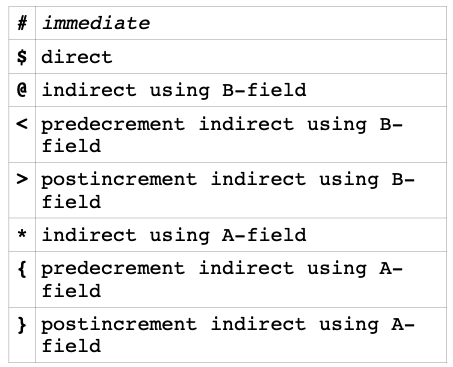
\includegraphics[scale=0.4]{image/modeAdressage.png}
                    \caption{Liste des différents modes d'adressage}
                \end{figure}
        \end{itemize}
        
        \paragraph{}Un guerrier peut écrire dans une case mémoire précédemment occupée par l'instruction d’un adversaire. Ainsi, un guerrier peut exécuter une instruction déposée par un autre à l'endroit où il se situe dans la mémoire. L'objectif va être de poser des bombes ( représentées par la ligne d'instruction DAT) dans la mémoire afin que des guerriers les exécutent et meurent.
        Lors d’une instruction SPL, le guerrier « sépare » ses tâches à exécuter et créer un nouveau processus. Si le guerrier A a l’instruction 1 et le guerrier B l’instruction 2, avant le SPL l’ordre d’exécution est 1|2|1|2 etc. Après l’exécution de l’instruction SPL, le guerrier A a un nouveau processus exécutant l’instruction 1’ et l’ordre d’exécution est maintenant 1|2|1’|2|1|2|1’|2 etc.\\
        Un combat fait participer au moins deux guerriers et le nombre maximal de guerriers présents dépend du type de tournoi auquel ils participent. Dans ce projet, nous avons utilisé les paramètres classiques d’exécution, soit un nombre d’instructions maximum de 100 pour un guerrier ainsi qu’un coresize de 8000.

        \newpage
        \paragraph{}Pour donner un exemple, voici le code d'un guerrier très basique appelé "Dwarf" : 
            \begin{center}
                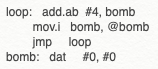
\includegraphics[scale=1]{image/dwarf.png}
            \end{center}
        La première instruction ajoute 4 au champ B de bomb.\\
        La deuxième copie la ligne bomb, n cases après bomb ; n étant le nombre indiqué par le champ B de bomb.\\
        La troisième demande au programme de revenir à la première instruction.\\
        La quatrième tue tout programme exécutant cette ligne, c'est la ligne bomb.
        
    \subsection{Présentation du sujet du projet}
        \paragraph{}Etant donné que l'écriture à la main d'un guerrier est très fastidieuse et que la modification d'une seule ligne d'un guerrier déjà existant peut le rendre inefficace, des joueurs ont développé des algorithmes d'évolution permettant de générer  des guerriers de manière évolutive. Pour ce projet, l'objectif était double : partir d'un article expliquant un algorithme d'évolution (voir Analyse de l'existant), le programmer et ensuite l'améliorer, ainsi qu'implémenter un système permettant un suivi du niveau des guerriers au cours des différentes exécution de l'algorithme en fonction des paramètres d'entrée.
        
    \subsection{Analyse de l'existant}
        \subsubsection{An Evolutionary Approach Generates Human Competitive Corewar Programs, de Barkley Vowk, Alexander Wait, Christian Schmidt}
            \paragraph{}Cet article est l'oeuvre de trois personnes que sont Barkley Vowk, Alexander (Sasha) Wait, Christian Schmidt ; les deux premiers étant des chercheurs universitaires respectivement de l'Université d'Alberta au Canada et de l'université d'Harvard aux États-Unis. Ils décrivent dans cet article un algorithme d'évolution permettant la génération de guerriers compétitifs pour Corewar.\\
            
            Dans un premier temps, ils expliquent les données qu'un guerrier possède et sur lesquelles il est possible de faire marcher l'évolution. En effet, les guerriers possèdent trois types de données dans leur code, que sont les instructions (une par ligne), les modifieurs (2 par ligne) et les techniques d'adressage de ces modifieurs (également deux par ligne). De plus, ils explicitent une méthode permettant de réaliser des statistiques sur les données des guerriers afin de produire la génération zéro de l'algorithme. Il est possible de calculer des probabilités qu'une instruction apparaît dans le code d'un guerrier suivant ses instructions antérieures.\\
            
            Enfin, ils expliquent la méthode utilisée pour l'évolution des guerriers. L'évolution se base sur une première génération produite à partir des statistiques générées précédemment. On fait combattre ces guerriers et on applique ensuite des mutations aléatoires à une certaine proportion de ces guerriers ainsi que des fusions entre plusieurs guerriers. Une fois ces nouveaux guerriers obtenus, on les fait combattre afin de ne conserver que les meilleurs et ainsi de suite.

        \newpage
        \subsubsection{Simulateur de MARS}
            \paragraph{}Il existe différents simulateurs de MARS mis à disposition des développeurs. En début de projet, nous avions choisi d'utiliser le simulateur Exhaust permettant de lancer des guerriers déjà compilés dans MARS et d'en ressortir les résultats du combat. Nous utilisons finalement Exmars, qui est une version améliorée d'Exhaust et qui permet notamment de lancer directement des guerriers codés en Redcode, le programme se chargeant de les compiler pour pouvoir les lancer dans MARS. Cependant Exmars reste un vieux logiciel que l'on a dû adapter et corriger pour l'utiliser dans notre programme. Exmars a été créé en prenant des parties d'Exhaust et Pmars, exhaust étant un très bon simulateur de combat en Redcode et pmars qui un très bon parseur de Redcode.
            
        \subsubsection{La base de données de guerriers}
            \paragraph{}Nous avons pu récupérer une base de données de plus de 1000 guerriers sur le site officiel de Corewar dont les guerriers du top 50. Cette base de données nous permet de générer des statistiques à partir d'un nombre important de guerriers déjà existant.

\newpage
\section{Les besoins}
    Pour le projet, il nous a fallu dégager les besoins fonctionnels et non fonctionnels du programme que nous allions réaliser.
    \subsection{Les besoins fonctionnels}
        Nous avons pu, après discussions avec notre client Mr Boussicault, faire ressortir les besoins fonctionnels suivant qui seront nécessaires pour l’algorithme d’évolution ainsi que pour l’outil de suivi des différentes exécutions. Pour l'algorithme d'évolution : implémenter une interface entre le simulateur (ExMars) et notre algorithme, implémenter un convertisseur entre les guerriers Redcode et la structure de guerrier du simulateur, pouvoir générer des statistiques concernant les instructions des guerriers, générer des guerriers à partir de statistiques, réaliser des combats et pouvoir récupérer le score d’un guerrier à l’issue d’un combat, modifier un guerrier, programmer un algorithme d’évolution, pouvoir modifier les paramètres d’exécution de l’algorithme. Pour le suivi des résultats entre les différentes exécutions : stocker en mémoire les paramètres d’exécution ainsi que le score du guerrier généré correspondant.\\
        \begin{itemize}
            \item Après avoir choisi le simulateur de MARS que nous allions utiliser, ici Exmars, il faut implémenter un module qui fonctionne comme une interface entre notre algorithme d’évolution et le simulateur. En effet, il faut que nous puissions être assez libres du choix du simulateur utilisé et que nos fonctions ne dépendent pas de ce dernier. L’interface est juste un intermédiaire entre les fonctions déjà implémentées dans le simulateur et les autres modules du logiciel. \\

            \item Les guerriers sont codés en Redcode et le simulateur utilise une structure de données particulières pour stocker ces informations. Le second besoin est donc d’implémenter un convertisseur de données. Il est nécessaire de pouvoir passer d’un guerrier « Redcode » en guerrier « ExMars » et vice-versa de manière rapide et claire. Passer du Redcode vers ExMars pour pouvoir utiliser les guerriers que nous allons récupérer sur internet ou que nous allons générer et d’Exmars vers le Redcode pour pouvoir stocker les guerriers que nous allons générer dans des fichiers texte. \\
            
            \item Pour établir une première génération de guerriers à partir de laquelle l’algorithme va effectuer les évolutions, nous avons besoin de statistiques concernant les instructions utilisées dans les guerriers codés à la main, leur pourcentage d’apparition en fonction de(s) l’instruction(s) précédente(s). Ainsi, ces statistiques doivent être générées au moins une fois et si le dossier est déjà présent leur re calcul n’est pas nécessaire. \\
            
            \item Il faut maintenant créer des guerriers à partir des statistiques calculées. C’est de ces guerriers que va pouvoir commencer l’évolution et aboutir sur des guerriers performants. \\
            
            \item Une des fonctionnalités essentielle du logiciel est de pouvoir réaliser des combats et de récupérer le score des guerriers présents. Une fonction permettant l’exécution des combats dans le simulateur ExMars va être implémentée ainsi qu’une autre permettant de récupérer le score. Ces combats permettent de tester l’efficacité des guerriers et d’effectuer un classement par le score afin de ne conserver que les meilleurs guerriers de chaque génération. \\
            
            \item Le besoin suivant est de pouvoir modifier un guerrier généré en choisissant la manière dont cela est fait. Pour faire évoluer la qualité globale des guerriers, il faut pouvoir améliorer un guerrier déjà existant et non pas seulement rajouter de nouveaux guerriers. \\
            
            \item Le travail principal du projet consiste en la programmation d’un algorithme d’évolution qui doit générer des guerriers performants. Pour cela, nous allons utiliser les fonctionnalités précédemment décrites. Nous allons donc créer la génération 0, effectuer des combats, modifier les guerriers en conséquence des scores obtenus. Il va être important de définir les paramètres modifiables d’un guerrier, voire ci-après, et de programmer les fonctions correspondantes. De plus, il peut être intéressant de pouvoir fusionner des guerriers. \\
            
            \item Il va également falloir définir des paramètres sur lesquels jouer avec notre algorithme d’évolution. On sait qu’un guerrier se compose de lignes de code, chacune étant une instruction suivie d’un modifieur et de deux valeurs avec un mode d’adressage. Cela nous fait déjà six champs sur lesquels interagir pour le code du guerrier. De plus, le nombre de lignes de code d’un guerrier n’est pas fixé. Il peut être intéressant de modifier cela aussi. \\
            
            \item Concernant le suivi des différentes exécutions de l'algorithme, il nous est nécessaire d'avoir une sauvegarde au moins au format texte des paramètres utilisés pour exécuter l'algorithme ainsi que le score obtenu par le guerrier généré.\\
        \end{itemize}

    \subsection{Les besoins non-fonctionnels}
    \begin{itemize}
        \item Les guerriers générés par l'algorithme d'évolution doivent battre les guerriers de la génération zéro et chaque génération doit être plus efficace que la précédente.\\
        
        \item Les statistiques que nous allons générer pour la création de la génération zéro se doivent d’être réalisées sur un nombre de guerriers conséquents. Il faut donc constituer une base de données d’au moins 500 guerriers à partir du site internet officiel de Corewar.\\
        
        \item L'exécution de l'algorithme doit pouvoir se faire en moins d'une heure avec 1000 générations.
        
    \end{itemize}

\newpage
\section{L'architecture et le logiciel}
    \subsection{Les réalisations}
        Notre programme se compose de trois modules principaux, sur lesquels nous allons revenir ci-après, d'un module existant qui est Exmars et d'un dernier module, utils, regroupant des fonctions souvent utilisées mais n'ayant pas spécialement de rapport avec le projet.
        
        \subsubsection{L'interface entre notre programme et Exmars (mars-interface)}
            \begin{enumerate}
                \item \textbf{La traduction des guerriers codés en Redcode en structure compréhensible par Exmars, et inversement (Redcode-switch.c)}
                    \paragraph{} Ce fichier contient deux fonctions qui nous permettent de réaliser ces deux opérations. Red\_to\_warrior traduit un guerrier codé en Redcode en structure warrior d'Exmars à partir de sa fonction assemble\_warrior. Print\_warrior permet de partir de la structure warrior et de recopier les instructions du guerrier ligne par ligne dans un fichier Redcode. 
                    \bigskip
                
                \item \textbf {Les méthodes de modification et d'accès aux guerriers (interface.c)}
                    \paragraph{} Nous avons codé un certain nombre de fonctions permettant d'accéder et de modifier des guerriers, dont la structure est précisée dans Exmars. Cela nous permet notamment de ne pas avoir à communiquer directement avec Exmars depuis l'algorithme d'évolution pour une meilleure maintenabilité et de permettre à notre algorithme de ne pas dépendre d'Exmars si jamais on souhaite changer de simulateur de MARS. Ce fichier se compose essentiellement de getter et de setter sur la structure warrior\_struct. 
                    \bigskip
                
                \item  \textbf {La réalisation des matchs/batailles entre les guerriers et la récupération des scores de combat (simple-interface.c)}
                    \paragraph{} C'est dans ce fichier que se trouve la partie la plus importante pour notre algorithme d'évolution. Il permet, en effet, de gérer ce qui se réfère à MARS, aux combats des guerriers et au calcul du résultat final de l'algorithme. 
                    \bigskip
                    
                    La fonction principale est do\_battle, qui sera appelée tout au long de l'exécution de l'algorithme d'évolution. Elle se charge d'initialiser la structure Mars d'Exmars à partir des guerriers qu'on lui donne. Ensuite, elle va réaliser un certain nombre de matchs suivant le paramètre correspondant entré par l'utilisateur. Et enfin elle va renvoyer les survivants  des différentes batailles, dont le nombre est également fixé par l'utilisateur, qui correspond aux guerriers ayant eu la meilleure moyenne de score. 
                    \bigskip
                    
                    La fonction get\_final\_score sera aussi importante pour le calcul de l'efficacité de l'algorithme d'évolution sur lequel nous reviendrons plus tard. 
                    \bigskip
                    
            \end{enumerate}
        \newpage
        \subsubsection{L'algorithme d'évolution (evolution-algorithm)}
            \begin{enumerate}
                \item \textbf {Le paramétrage (evolution-parameters.c) :} 
                    \paragraph{}Les structures evolution\_params et changing\_param ont été créées afin de stocker les différents paramètres choisis par l'utilisateur pour l'algorithme d'évolution. Une majorité des champs de evolution\_params sont du type structure changing\_param, dont les deux principaux champs sont level et value. Cela nous permet, pour les champs correspondant de evolution\_param, de stocker des valeurs différentes, avec value, en fonction de la génération à laquelle on se situe durant l'exécution de l'algorithme d'évolution, avec level. On peut ainsi mieux contrôler notre évolution. Par exemple si l'on souhaite réduire le nombre de guerriers mutés au cours de l'évolution ou si l'on souhaite réduire la probabilité de fusion entre deux guerriers etc. 
                    \bigskip
                    
                    Ces paramètres sont définis par l'utilisateur dans le fichier json evolution-params. On réalise ensuite le parsage du fichier et la récupération des différentes valeurs dans la structure evolution\_params. En état, les paramètres de contrôle de notre algorithme d'évolution sont les suivants  : 
                    
                    \bigskip
                    \begin{itemize}
                        \item "version" : Le numéro de version de notre algorithme d'évolution avec les paramètres indiqués. Si l'on souhaite relancer l'algorithme toujours avec les mêmes paramètres, il ne faut pas toucher à ce paramètre. Cependant, si on modifie les paramètres il convient d'incrémenter ce paramètre qui nous servira pour le calcul des résultats à la fin du programme, expliqué ci-après.
                        \item "generations" : Le nombre de générations sur lequel l'algorithme va itérer.
                	    \item "battles\_by\_generation" : Le nombre de batailles que vont effectuer les guerriers dans MARS pour chaque génération.
                    	\item "num\_warriors" : Le nombre de guerriers produits par génération
                    	\item "A\_value\_modifier\_min" / "A\_value\_modifier\_max" / "B\_value\_modifier\_min" / \newline"B\_value\_modifier\_max" : La changement de valeur minimum et maximum que peuvent subir les valeurs A et B dans les instructions des guerriers lors d'une mutation.
                    	\item "survivors" : La proportion de guerriers survivants et passant d'une génération à une autre.
                    	\item "mutations" : La proportion de guerriers qui vont recevoir une mutation lors d'une nouvelle génération.
                    	\item "breeding" : La proportion de guerriers qui vont être fusionnés lors d'une nouvelle génération.
                    	\item "fresh" : La proportion de guerriers qui vont être générés à partir du fichier des statistiques réalisées.
                    	\item "old" : La proportion de guerriers qui vont être récupérés depuis des survivants d'anciennes générations qui ont été éliminés précédemment.
                    	\item "p\_mutation\_line" : La probabilité qu'une ligne d'instruction donnée d'un guerrier soit modifiée lors d'une mutation.
                    	\item "p\_mutation\_field" : La probabilité qu'un champ donné (valeur, modifier...) soit modifié lors de la mutation d'une ligne d'instruction d'un guerrier.
                    	\item "breed\_length\_min" / "breed\_length\_max" : Le nombre de lignes minimum et maximum d'un guerrier qui vont être remplacés par les lignes d'un autre guerrier lors d'une fusion entre deux guerriers.
                    	\item "generator\_path" : Le chemin du dossier sur lequel calculer les statistiques. 
                    	\item "generator\_depth" : La profondeur que l'on souhaite explorer pour la génération des statistiques. 
                    \end{itemize}
                    
                    \bigskip
                    Il est important de noter que la somme des valeurs des champs "survivors", "mutations", "breeding", "fresh" et "old" doit être égale à 1. Si cette condition n'est pas respectée le nombre de guerriers modifiés ou générés dépasse le nombre de guerriers que l'on souhaite par génération et l'algorithme ne peut être exécuté. \\
                    
                    \begin{figure}[!h]
                    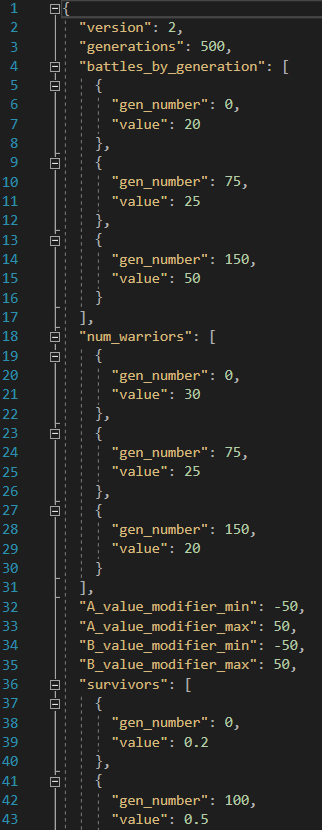
\includegraphics[height=17cm]{image/ParametresPartie1.png} 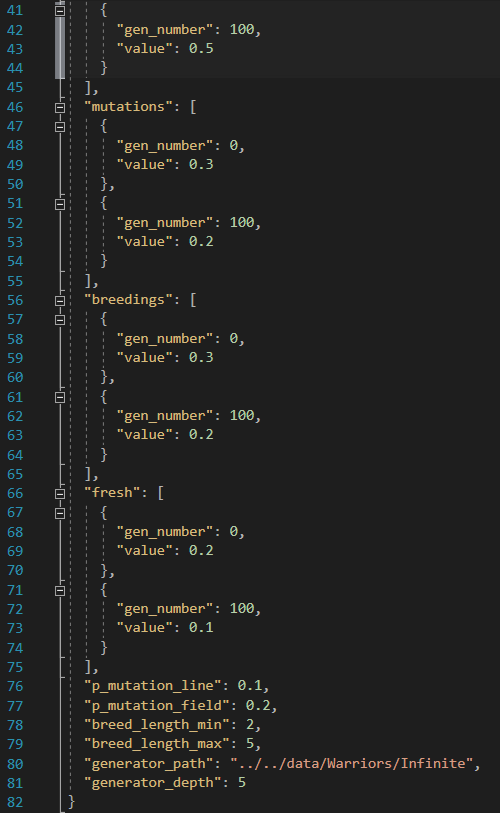
\includegraphics[height=17cm]{image/ParametresPartie2.png}
                        \caption{Fichier json contenant les paramètres d'exécution}
                    \end{figure}
                    
                
                \newpage
                \item \textbf {Le déroulement (evolution-algorithm.c) :}
                    \paragraph{}Au début de l'algorithme, nous mettons à jour le nombre de guerriers survivants, mutés, fusionnés et générés à partir des statistiques, qui vont être pris en compte après les batailles entre les guerriers de la génération courante. Ensuite, nous allons effectuer ce qui suit un certain nombre de fois, qui correspond au nombre de générations souhaitées par l'utilisateur. Nous effectuons les batailles entre les guerriers grâce à la fonction do\_battle(), expliquée plus tôt, qui renvoit un tableau de guerriers, les survivants. Nous allons ensuite appliquer des mutations et des fusions expliquées ci-après, sur les survivants suivant les paramètres récupérés plus tôt, puis nous générons de nouveaux guerriers "frais" à partir des statistiques. Cela permet notamment de limiter le sur-apprentissage des guerriers. Ces différentes étapes vont se répéter suivant le nombre de générations voulues. Enfin, l'algorithme renvoie les meilleurs guerriers de la dernière génération, correspondant aux survivants de la dernière bataille.
                    \\
                    
                    En ce qui concerne les mutations et fusions appliquées aux guerriers : \begin{itemize}
                        \item Une fonction de mutation parcourt toutes les lignes de code du guerrier et pour chaque ligne, génère un nombre pseudo-aléatoire à comparer à la probabilité de modifier une ligne (passée en paramètre de l'algorithme). Si le nombre généré est inférieur à la probabilité alors on refait cette opération pour chaque champ de la ligne. Si le nombre est de nouveau inférieur à la probabilité alors on modifie le champ en question aléatoirement, suivant les valeurs qu'il accepte.
                        \item Ensuite, il y a une fonction permettant de modifier la taille d'un guerrier. En effet, on peut supprimer des lignes ou en ajouter des nouvelles. S'il y a un ajout de lignes alors celles-ci sont générées aléatoirement.
                        \item Enfin, il y a la possibilité de fusionner deux guerriers. Cela consiste à remplacer un groupe de lignes de code d'un guerrier A par un groupe de même taille de lignes de code d'un guerrier B.
                    \end{itemize}
                    \bigskip
                \item \textbf{Le calcul du score de l'algorithme (scoring.c) :}
                    \paragraph{}Une fois les survivants de la dernière génération récupérés, nous allons calculer le score de l'algorithme d'évolution suivant les paramètres que l'utilisateur lui a donnés. La fonction qui calcule cela se déroule ainsi : \\
                
                    On fait combattre les guerriers un millier de fois afin d'obtenir un score de combat stable. Ensuite, on réduit ce nombre afin d'avoir un score précis au point (c'est-à-dire qu'un guerrier donné aura la majorité du temps le même score +/- 1). Le score est obtenu sur le meilleur des guerriers de l'algorithme d'évolution contre un groupe de guerriers prédéterminé. Dans ce cas précis on utilise deux des guerriers du top 50 de Corewar, deux guerriers basiques et un bon guerrier. Le score est calculé selon la métrique officielle de Core War, avec N le nombre de guerriers et W le nombre de survivants à la fin d'un combat : N*(N-1)/W (avant d'être réduite). Ainsi sont regardées les données suivantes: la quantité de victoire d'un guerrier (être le seul survivant à l'issu de tout les tours), et les quantités d'égalités à plusieurs, en prenant en compte qu'il est préférable de finir à égalité à 2 guerriers qu'à 5.\\
                    
                \item \textbf{L'affichage des résultats :}
                    \paragraph{} À la fin de notre programme, un fichier json va être généré par la fonction print\_results à partir du paramètre "version" du fichier evolution-params expliqué plus tôt. Le fichier généré est de la même structure que le fichier json des paramètres avec deux champs supplémentaires, que sont "time\_tested" et "score". Le premier permet de stocker le nombre de fois que l'algorithme a été lancé avec les paramètres indiqués. Nous souhaitons insister sur l'importance de l'attribut "version", qui nous permet de vérifier simplement que la version est correspondante plutôt que comparer toutes les valeurs du fichier des paramètres. Cet attribut, "time\_tested", s'incrémentera si la valeur du champ "version" a déjà été utilisée. L'attribut "score" permet quant à lui de stocker la moyenne des scores obtenus avec l'algorithme d'évolution suivant la version renseignée. À chaque version des paramètres utilisés correspond un fichier résultats correspondant.
                    
                    \begin{figure}[!h]
                    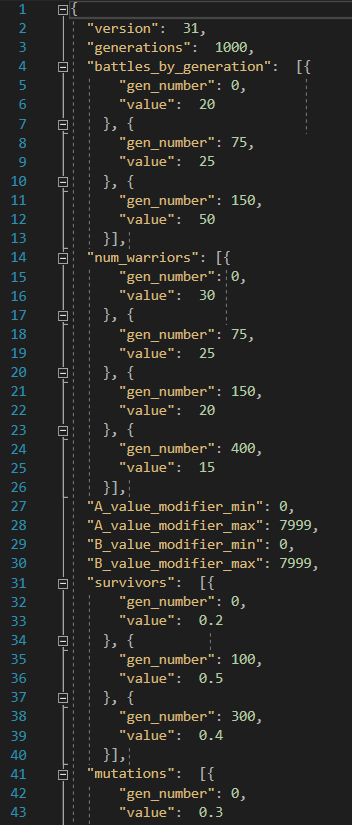
\includegraphics[height=15cm]{image/Resultats1.png} 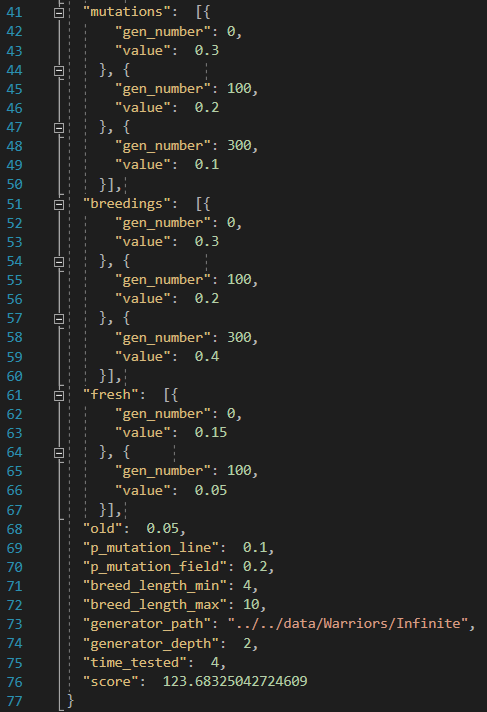
\includegraphics[height=15cm]{image/Resultats2.png}
                        \caption{Fichier json contenant les résultats de l'exécution avec les paramètres de la version 31}
                    \end{figure}
            \end{enumerate}
        \newpage
        \subsubsection{La génération de statistiques sur les instructions de plus de 1000 guerriers (analyser)}
            \paragraph{} Pour la génération zéro de nos guerriers et pour ne pas tomber dans le piège du sur-apprentissage pour nos guerriers pendant l'algorithme d'évolution, il nous a fallu trouver un moyen de les générer d'une manière aléatoire mais cohérente. Pour cela, nous nous sommes aidés de la méthode décrite dans l'article présentant un algorithme d'évolution pour Corewar [5]. 
            \bigskip
            
            Nous avons deux parties distinctes que sont la génération des statistiques et la génération de guerriers à partir de ces statistiques.
            \begin{itemize}
                \item Le fichier analyser.c a pour but de proposer des outils pour analyser un panel de guerriers et d'en sortir des statistiques. Nous pouvons paramétrer ces statistiques grâce à une profondeur. Pour une profondeur de deux, qui est la profondeur minimale souhaitée, nous pouvons analyser l'instruction d'un guerrier et la précédente, et ainsi de suite pour des profondeurs supérieures. Le but de cette profondeur est d'obtenir une précision plus importante sur les statistiques. En ce qui concerne le calcul des statistiques, nous mettons les probabilités de trouver une instruction, après n autres instructions données, dans un tableau à (n+1) dimensions. Une fois les  statistiques terminées, un fichier stats[n+1].json sera généré dans le même dossier que les guerriers.
                \item Pour ce qui est de la génération des guerriers à partir des statistiques, cela se passe dans le fichier generator.c. Pour cela, nous   utilisons les statistiques calculées précédemment et générons un guerrier basique 
                aléatoire en fonction de la probabilité de présence des instructions.
            \end{itemize} 
        
        \subsubsection{La parallélisation de code}
            \paragraph{} Nous avons pu observer lors de la génération des guerriers et du calcul des résultats que le programme va effectuer beaucoup d'opérations, notamment des combats. Ces combats étant indépendants les uns des autres, il est possible de gagner du temps en utilisant la programmation parallèle afin que plusieurs threads se partagent l'exécution des différents combats. Pour cela, nous avons utilisé  OpenMP. Cet outil de parallélisation nous offre une solution efficace (par rapport à une version séquentielle) et des gains immédiats de manière simple. Il existe néanmoins d'autres techniques et outils de parallélisation qui peuvent se montrer plus efficaces. Évidemment, dans toute architecture parallèle il faut faire attention aux accès concurrents des threads aux mêmes variables, d'autant plus que les structures manipulées sont essentiellement des structures de pointeurs. Ainsi il est apparu évident de recopier certaines variables plutôt sensibles pour chaque thread (les warriors\_s qui contiennent notamment leur position dans mars et d'autres informations sensibles) et de partager une variable contenant les résultats des batailles qui seront accédés de manière atomique. Puis lorsque les threads auront terminé leur travail, cette variable sera attribuée au champ de mars qui convient.
            \paragraph{} De cette manière, on gagne un temps considérable. L'exécution du programme en séquentiel sur 50 générations prend entre deux et trois minutes et sur 500 générations entre 20 et 25 minutes. Dans cette version parallélisée avec quatre threads, le programme s'exécute respectivement en moins d'une minute et en environ onze minutes. Évidemment les machines du crémi en salle 008 offrent des performances supérieures de par leurs caractéristiques. Il est possible d'utiliser jusqu'à 48 threads sur ces machines. La vitesse d'exécution du programme devient alors très intéressante : exécution sur 3000 générations en environ dix minutes.

        \newpage
        \subsection{L'architecture}
            \paragraph{}L'architecture de notre programme se décompose en quatre principaux modules dont un déjà existant qu'est Exmars.\\
            
            \paragraph{} Le module Analyser permet la création de statistiques sur les instructions de notre base de données de guerriers ainsi que la création de la génération zéro et de nos guerriers "frais" au cours de l'évolution.\\
            Ensuite le module Exmars est la librairie de notre simulateur de MARS qui contient notamment les structures des guerriers et de MARS. Elle possède également toutes les fonctions nécessaires à la réalisation des batailles entre les guerriers, du calcul des scores, de la conversion des guerriers codés en Redcode en structure Exmars etc. \\
            Le module Mars-Interface est une interface entre notre algorithme d'évolution et Exmars. Cette interface possède de nombreux getter et setter ainsi que des fonctions pour la réalisation de matchs personnalisés et la récupération des scores. \\
            Enfin, le module principal est Evolution-Algorithm, qui se compose de l'algorithme d'évolution, des différentes structures pour son paramétrage, des différentes fonctions de mutations des guerriers ainsi que du main.
            
        \begin{figure}[!ht]
            \centering 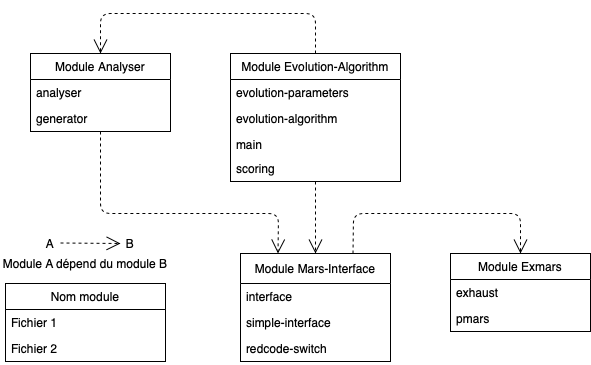
\includegraphics[scale=0.7]{image/Dependance.png}
            \caption{Schéma de dépendance entre les modules principaux}
        \end{figure}
        
        \paragraph{} Le module de l'algorithme d'évolution dépend de Analyser et de Mars-Interface, qui lui même dépend de Exmars.

        \newpage
        \paragraph{} Nous souhaitons également revenir sur l'exécution de notre algorithme d'évolution depuis le main. \\
        Notre programme débute par la récupération du fichier json de paramétrage de l'algorithme d'évolution. Ce fichier est parsé et la structure evolution-params est initialisée à partir des valeurs pour la génération zéro. \\ 
        Ensuite notre pool de guerriers est créé à partir des statistiques que nous avons générées. Ce pool correspond aux guerriers de la génération zéro de notre algorithme. \\ 
        Nous appelons ensuite notre algorithme d'évolution avec ses paramètres initialisés et le pool de guerriers. La boucle principale de l'algorithme va s'effectuer un certain nombre de fois, correspondant au nombre de générations souhaitées. Dans cette boucle, on met tout d'abord à jour les paramètres de notre algorithme d'évolution suivant la génération à laquelle on se trouve. Ensuite, on réalise les batailles entre les guerriers,  suivant le nombre indiqué en paramètre et on récupère les meilleurs guerriers suivant un nombre souhaité. On va ensuite réaliser les différentes mutations et fusions par rapport aux proportions indiquées dans les paramètres d'évolution et enfin on génère de nouveaux guerriers "frais" à partir des statistiques. On recommence ainsi une nouvelle boucle. 
        \begin{figure}[!ht]
            \centering 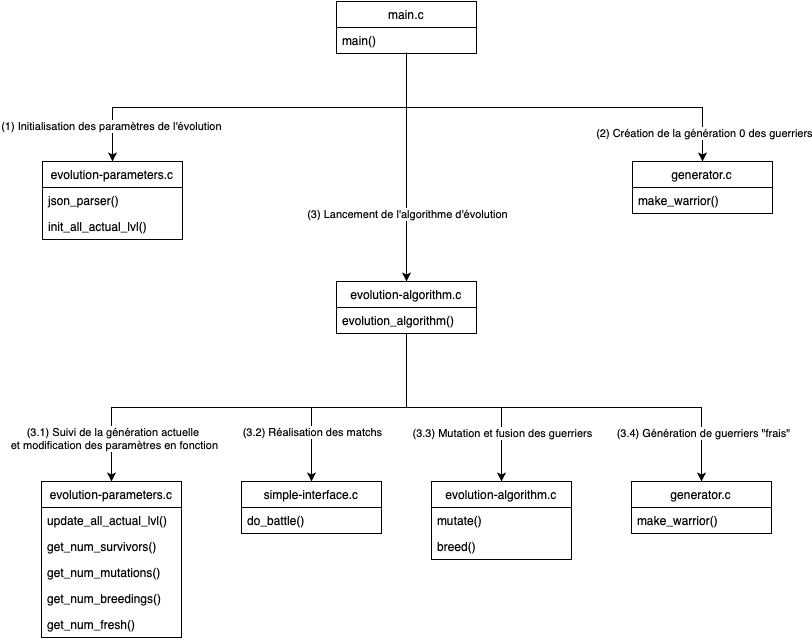
\includegraphics[scale=0.6]{image/mainAlgo.png}
            \caption{Schéma d'exécution de l'algorithme d'évolution depuis le main}
        \end{figure}

\clearpage

\section{L'analyse du fonctionnement et les tests}
    \subsection{Le déroulement du programme} 
        \paragraph{} Le fonctionnement de notre programme est le suivant : 
        \begin{itemize}
            \item L'utilisateur initialise les paramètres de l'algorithme d'évolution dans le fichier evolution-params.json présent dans le dossier "src". 
            \item On exécute ensuite le programme qui va réaliser les différentes évolutions en partant des guerriers de la génération zéro. Pour chaque génération, le nom du meilleur guerrier s'affiche sur le terminal. Le nom d'un guerrier se compose des noms de ses ancêtres, représentés par des nombres, séparés par un underscore. 
            \item A la fin du programme, le nom des guerriers retenus de la dernière génération s'affiche, suivi du calcul du score de l'algorithme. Ce score est récupéré de la manière suivante. On réalise un combat entre le meilleur guerrier de la dernière génération contre notre pool de test, constitué de deux guerriers du top 50, un bon guerrier et deux guerriers basiques, et on récupère le score de notre guerrier à l'issue d'un grand nombre de combats. 
        \end{itemize}
        Le principal objectif est de trouver les paramètres pour notre algorithme d'évolution qui permettront de générer le guerrier le plus performant.
        
    \subsection{Les test}
        \subsubsection{La comparaison des guerriers de plusieurs générations}
            \paragraph{} Afin de voir que notre algorithme d'évolution est réellement performant, il est utile de faire combattre les guerriers de la première génération contre les guerriers de la dernière. Si le programme est performant alors les guerriers produits par notre algorithme obtiendront un score supérieur comparé au score des premiers guerriers.\\
            Nous avons, par conséquent, effectué des combats entre trois guerriers de la première et trois de la dernière génération. Comme on peut voir dans la figure ci-après, le résultat est sans appel. Les trois guerriers générés par l'algorithme d'évolution battent les trois guerriers initiaux qui n'arrivent pas à survivre.
            \begin{figure}[!h]
                \centering 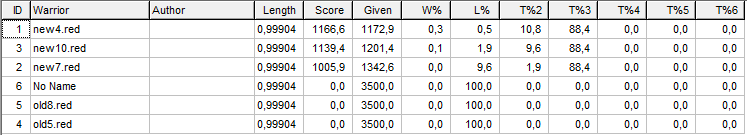
\includegraphics[scale=0.6]{image/test1.png}
                \caption{Tableau des résultats généré par le logiciel Corewin lors d'un combat de vérification}
            \end{figure}
        
        \subsubsection{La modification de la profondeur pour la génération des statistiques}
            \paragraph{} Ce test peut nous permettre de vérifier que la profondeur optimale pour le calcul des statistiques est bien cinq, comme indiqué dans l'article sur lequel nous nous sommes basés. Il consiste à exécuter notre programme avec des paramètres d'évolution identiques mais une profondeur pour les statistiques différentes. Nous constatons un score maximum pour notre algorithme d'évolution avec la profondeur cinq. \\ \\
            
            \newpage
            Les résultats obtenus sont les suivants : 
            \begin{itemize}
                \item Profondeur 2 : 101,3
                \item Profondeur 3 : 103,6
                \item Profondeur 4 : 101,6
                \item Profondeur 5 : 111,2
                \item Profondeur 6 : 96,3
                \item Profondeur 7 : 105,1 
            \end{itemize}
            
            \bigskip
            Après avoir testé une dizaine de fois avec les mêmes paramètres d'évolution mais des profondeurs de 2, 3, 4, 5, 6 et 7, on peut voir une nette amélioration pour la profondeur 5.\\
            
        \subsubsection{La modification du nombre de générations}
            \paragraph{} Avec ce test nous pouvons observer la corrélation qui peut exister, ou non, entre le nombre de générations pour l'algorithme d'évolution et la performance obtenu pour le meilleur guerrier de cette évolution. \\
            Après de nombreux tests nous avons pu observer que, en fonction des paramètres, plus le nombre de générations est important plus l'algorithme et performant et dans d'autres cas c'est l'inverse. Nous pouvons en conclure que les performances du guerrier généré dépendent tout de même des autres paramètres que l'on choisit pour l'évolution et pas seulement du nombre de générations.\\
            
        \subsubsection{Test relatif à l'impact du groupe de guerrier sur lequel les statistiques sont calculées}
            \paragraph{} Avec ce test nous pouvons observer les conséquences du changement du groupe de guerriers pour la génération 0 ainsi que les nouveaux guerriers au cours de l'évolution. \\
            Nous avons testé un groupe de guerriers différents pour les statistiques avec les guerriers du Top50 au lieu des 1000 guerriers issu d'Infinite et les résultats montrent que l'échantillon des 50 guerriers n'est pas suffisant pour faire une évolution efficace. En effet là où la meilleure configuration que nous avons trouvée a un score de 123,7 avec le groupe Infinite, la même configuration avec les statistiques du top50 a donné un score de 106,7. Il pourrait être intéressant d'avoir accès à un classement comportant un nombre de guerriers plus important que le top50 mais dont nous connaîtrions la qualité afin de parfaire ce test et comparer les résultats avec les mêmes conditions d'exécution.

\newpage
\section{Conclusion}
    \subsection{Bilan du projet}
        \paragraph{}Le projet touche à sa fin et le bilan nous semble plutôt positif. Les tests ont montré que nous avons réussi à implémenter un algorithme d'évolution fonctionnel et efficace. Nous avons défini de nombreux paramètres modifiables pour essayer d'obtenir la génération de guerriers la plus efficace possible. Nous avons également développé un moyen de suivre les résultats de notre algorithme suivant les paramètres que nous lui fournissons. 
    
    \subsection{Améliorations possibles}
    
    \paragraph{}Malgré ce bilan positif, il y a des éléments existants que nous aurions souhaité approfondir ou même créer de nouveaux éléments, mais pour lesquels le temps nous a manqués. \\
    Tout d'abord il serait possible d'implémenter d'autres algorithmes d'évolution présentés sur la page officielle de Corewar. Cela permettrait de comparer les résultats obtenus entre les différents programmes et de, peut-être, en ressortir un plus efficace que les autres. \\
    Il peut être intéressant aussi de calculer les statistiques à partir de différents groupes de guerriers. On pourrait donc observer l'impact réel de ces statistiques et des guerriers sur lesquels elles sont basées ainsi que du groupe de guerrier constituant la génération 0.\\
    Il aurait aussi pu être intéressant de permettre de forcer à conserver plusieurs "espèces" de guerrier lors de l'exécution, c'est à dire observer des similitudes dans le code et le comportement des guerriers et leur assigner différents groupes afin de pouvoir garder une certaine variété, mais nous n'avons pas vu comment faire et nous avons simplement implémenté le fait de faire revenir des guerriers précédemment éliminés.

\newpage
\section{Bibliographie}
    \begin{itemize}
        \item Documentation sur Corewar et le Redcode
        \begin{itemize}
            \item [1] John K. Lewis. \textbf{Corewars for Dummies}, (URL : \url{https://Corewar.co.uk/lewis/index.htm}) (Accédé en Janvier 2021).
            \item [2] Ilmari Karonen.  \textbf{Beginner's Guide to Redcode}, (URL : \url{https://vyznev.net/Corewar/guide.html}) (Accédé en Janvier 2021).\\
        \end{itemize}
        \item Simulateurs de MARS
        \begin{itemize}
            \item [3] Joonas Pihlaja.  \textbf{exhaust 1.9.2}, 27 Juillet. 2004,  (URL : \url{https://Corewar.co.uk/pihlaja/exhaust/index.htm}) (Accédé en Février 2021).
            \item [4] Martin Ankerl.  \textbf{Corewars Simulators Overview}, 29 Juilllet 2006,  (URL : \url{https://martin.ankerl.com/2006/07/29/corwars-simulators-overview/}) (Accédé en Février/Mars 2021). \\
        \end{itemize}
        \item Corewar et l'évolution
        \begin{itemize}
            \item [5] John Perry.  \textbf{Core Wars Genetics: The Evolution of Predation}, Janvier 1991,  (URL : \url{https://Corewar.co.uk/perry/evolution.htm}) (Accédé en Février 2021).
            \item [6] Terry Newton.  \textbf{Using Core Wars to Simulate Evolution}, 7 avril 2009,  (URL : \url{http://newton.freehostia.com/cwevol.html}) (Accédé en Février/Mars 2021).
            \item [7] Linus Thorsell.  \textbf{Evolving warriors}, 1 novembre 1999,  (URL : \url{https://Corewar.co.uk/thorsell/paper.htm}) (Accédé en Février/Mars 2021).\\
        \end{itemize}
        \item Présentation d'algorithme d'évolution pour Corewar
        \begin{itemize}
            \item [8] Barkley Vowk, Alexander (Sasha) Wait, Christian Schmidt. \textbf{An Evolutionary Approach Generates Human Competitive Corewar Programs}, 2004,  (URL : \url{https://Corewar.co.uk/vowk/alife9ac.pdf}) (Accédé de Janvier à Avril 2021).
        \end{itemize}
    \end{itemize}
\end{document}
